\label{sec:NuMUCCsel}

\par This chapter presents the two $\nu_{\mu}$ selections of the analysis; both are inclusive selections, but with different distributions. The first selection (sec \ref{ssec:NuMUCCsel:INC}) provides a pure, high-statistics sample of $\nu_{\mu}$s and the second selection (sec \ref{ssec:NuMUCCsel:constr}) is optimized to be used as a constraining tool in the $\nu_e$ analysis. 

\subsection{Variable Definitions}
\label{ssec:NuMUCCsel:sel:vars}

\par Below are a concise list of variables used in the $\nu_{\mu}$ selections. The variables are organized into \textit{slice} and \textit{track}-level descriptors, used for preselection and muon-candidate selection respectively. There is some redundancy between this list and the list in sec \ref{sec:nueselection:variables}, but this list below should serve as a quick reference to a reader of this chapter.

\par \noindent \textbf{Slice variables}: These variables generally describe the reconstructed neutrino interaction, i.e. the confluence of data gathered from all the PFParticles in the slice.
\begin{itemize}
    \item \emph{nslice}: number of neutrino slices identified by the SliceID (possible values are 0 or 1).
    \item \emph{n\_tracks\_contained}: number of tracks fully contained in the fiducial volume.
    \item \emph{reco\_nu\_vtx\_sce\_\{x,y,z\}}: Reconstructed, spacecharge-corrected neutrino interaction vertices in (x,y,z) coordinates (see fig. \ref{fig:numu_vtx}.
    \item \emph{topological\_score}: A machine-learned quantity that reflects the complexity and directionality of observable slice quantities. This variable has strong discriminating power between signal and cosmic-background (see \ref{fig:numu_topo_pid} (possible values are between 0 and 1).
    \item \emph{CRT Veto and Distance Tagger}: Tools provided by the cosmic ray tagger (see sec. \ref{sec:sliceID:CRT}).
\end{itemize}

\par \noindent \textbf{Track variables}: These variables specifically describe the reconstructed PFParticles; in interest to this selection are reconstructed track-like objects. 
\begin{itemize}
    \item \emph{trk\_sce\_\{start,end\}\_\{x,y,z\}}: Reconstructed, spacecharge-corrected start/end-points for the tracks.
    \item \emph{trk\_llr\_pid\_score}: The log likelihood ratio particle identification score (see sec. \ref{subsec:loglikelihoodpid}). This variable has strong muon-proton discriminating power (see fig. \ref{fig:numu_topo_pid}).
    \item \emph{trk\_score}: A machine-learned quantity that describes how `track-like' the reconstructed object is (possible values between 0 and 1).
    \item \emph{trk\_len}: The length of the reconstructed track (in cm).
    \item \emph{trk\_distance}: The distance from the start-point of the reconstructed track to the reconstructed neutrino vertex (in cm).
    \item \emph{pfp\_generation}: The generation of the PFParticle according to Pandora, i.e. how many parents the object on interest has in the slice.
\end{itemize}

\begin{comment}
\subsubsection{Backgrounds}
\label{sssec:NuMUCCsel:sel:bkgrnds}

\par Coming soon...

\subsubsection{Fiducial Volume and Spacecharge-Corrected Spacepoints}
\label{sssec:NuMUCCsel:sel:FVandSCE}

\par Coming soon...
\end{comment}

\begin{figure}
    \centering
    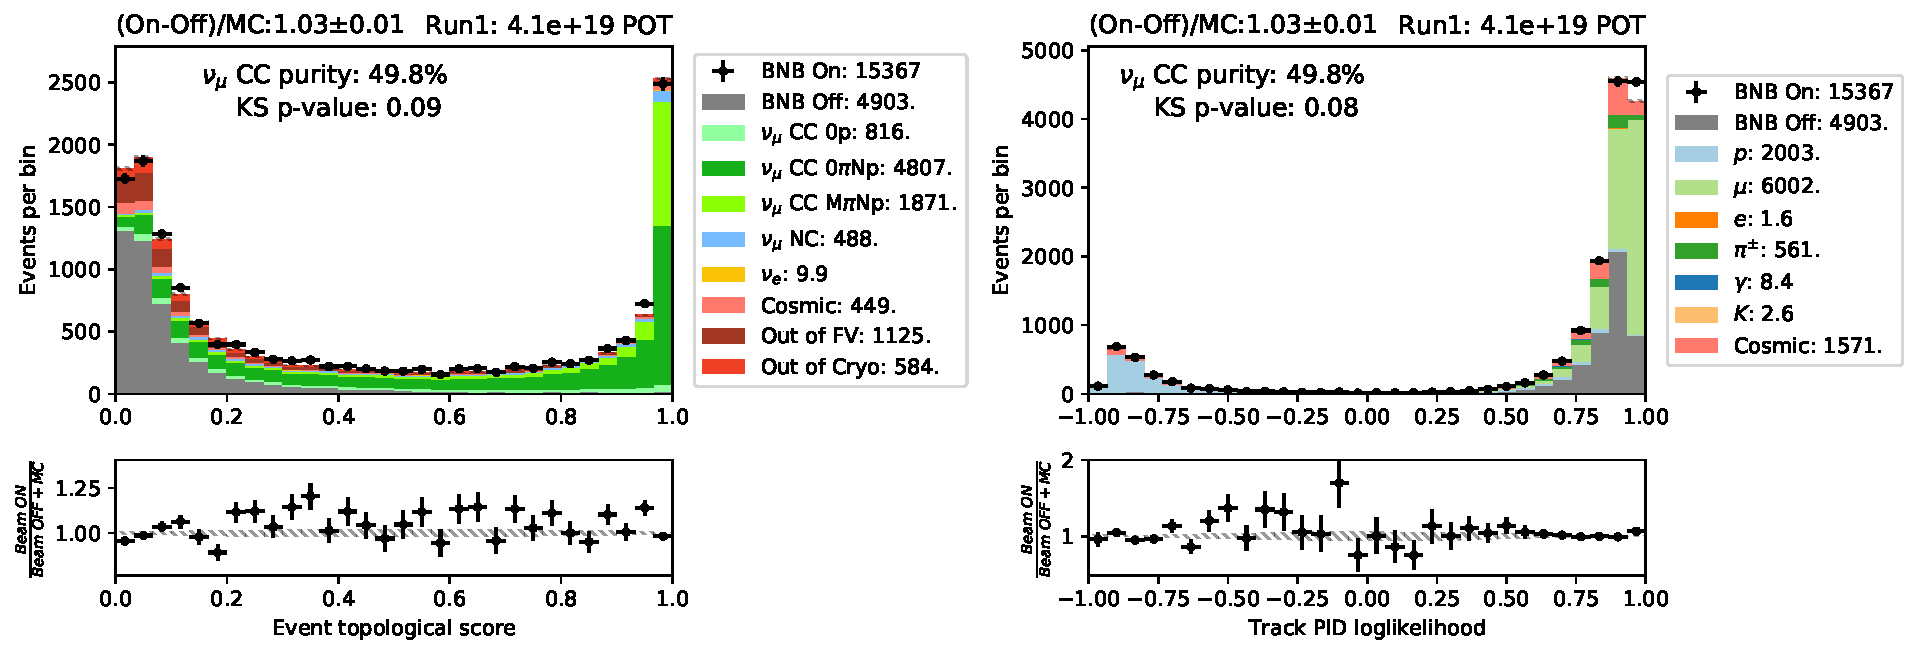
\includegraphics[width=\textwidth]{NuMuCCsel/Images/run1/numu_pret_run1.pdf}
    \caption{Caption}
    \label{fig:numu_topo_pid}
\end{figure}

\subsection{Inclusive Selection}
\label{ssec:NuMUCCsel:INC}

\subsubsection{Run 1}
\label{sssec:NuMUCCsel:INC:Run1}


\begin{figure}
    \centering
    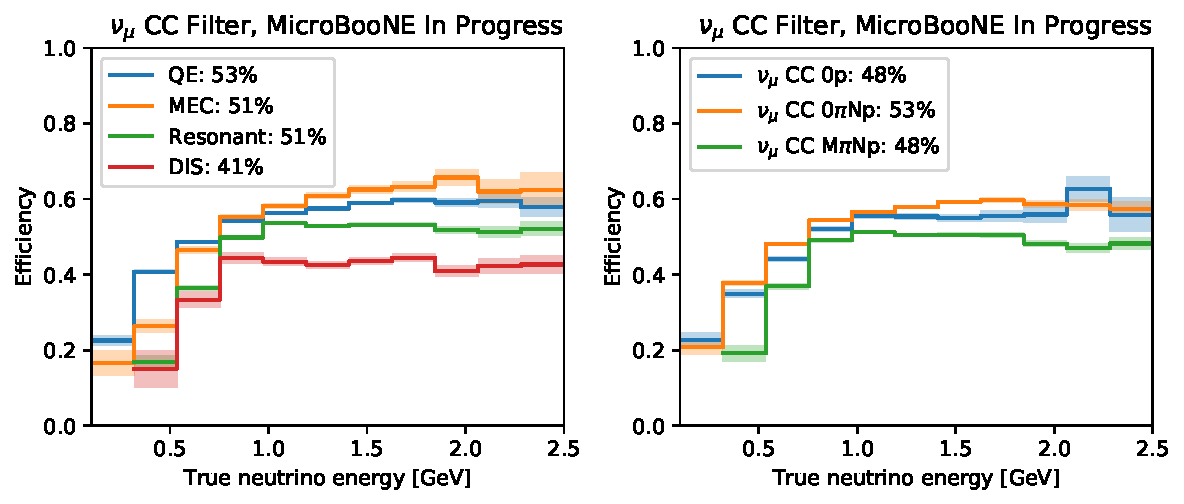
\includegraphics[width=0.85\textwidth]{NuMuCCsel/Images/run1/numu_efficiency_run1.pdf}
    \caption{Caption}
    \label{fig:numu_eff_r1}
\end{figure}

\begin{figure}
    \centering
    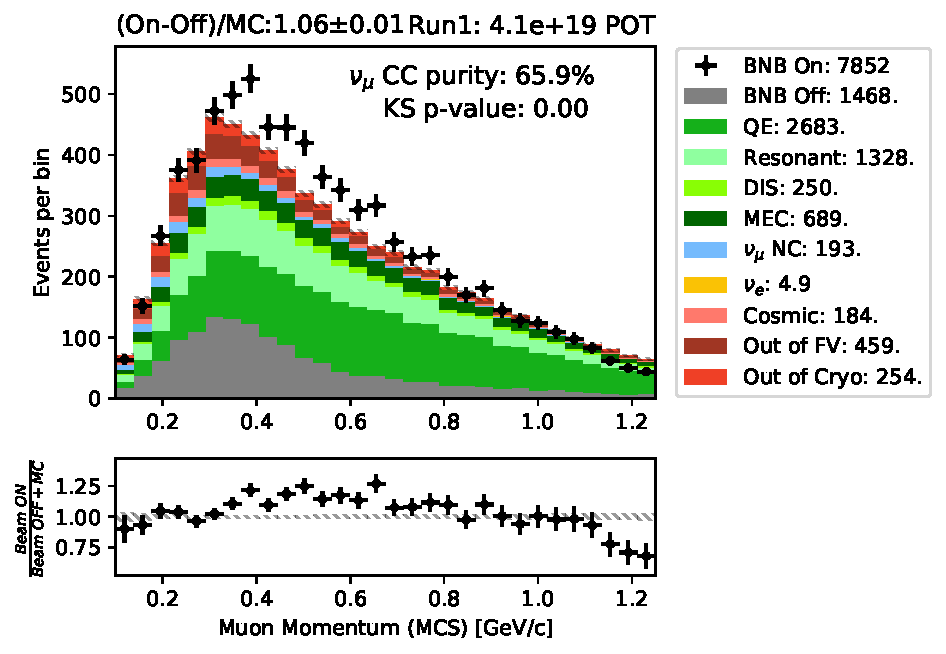
\includegraphics[width=0.495\textwidth]{NuMuCCsel/Images/run1/numu_mcsmom_run1.pdf} \hfill
    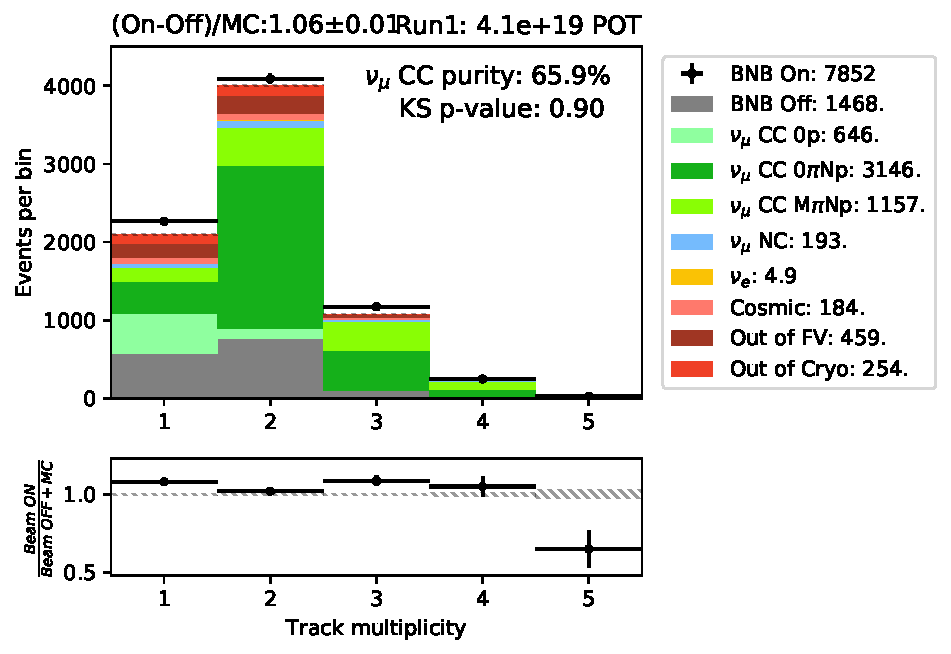
\includegraphics[width=0.495\textwidth]{NuMuCCsel/Images/run1/numu_vtxntrack_cat_run1.pdf}
    \caption{Caption}
    \label{fig:numu_mcs}
\end{figure}

\begin{figure}
    \centering
    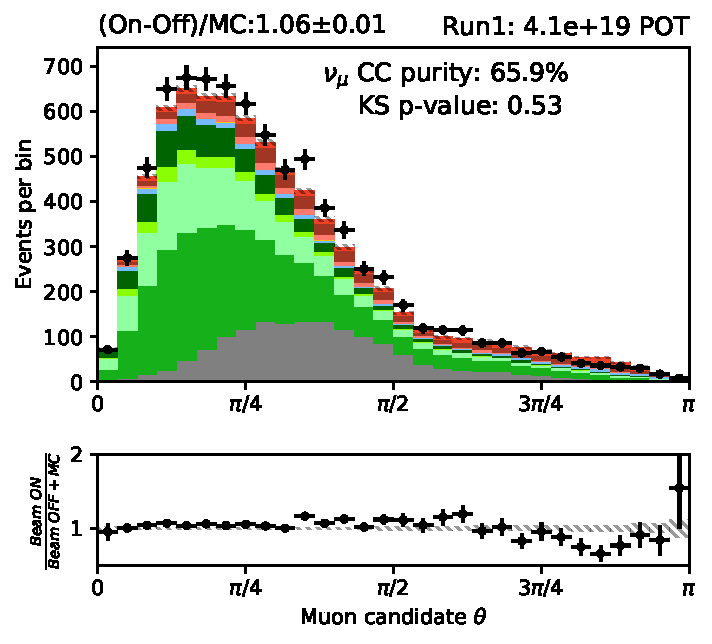
\includegraphics[height=6.5cm]{NuMuCCsel/Images/run1/numu_theta_run1.pdf} \hspace{2mm}
    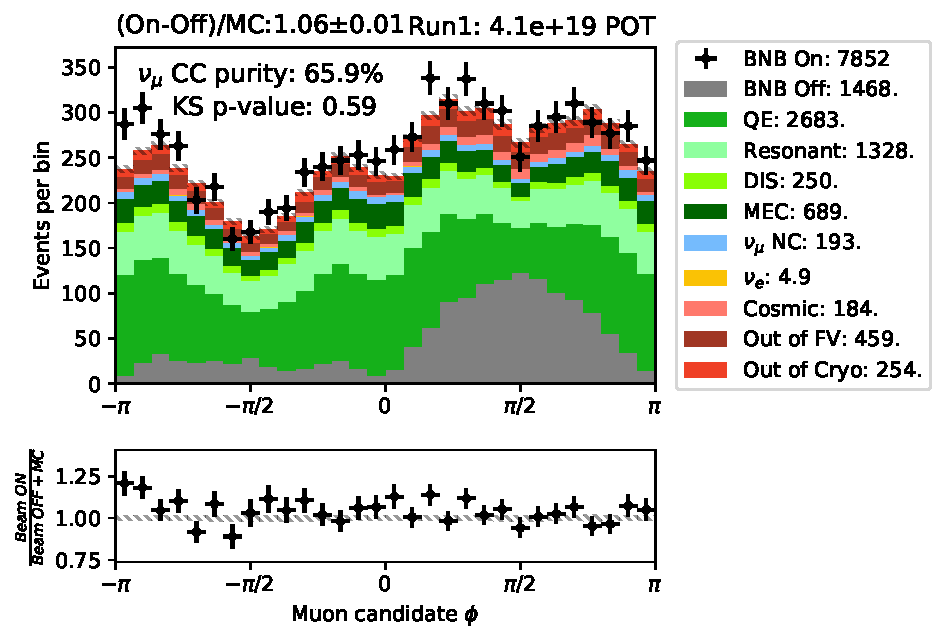
\includegraphics[height=6.5cm]{NuMuCCsel/Images/run1/numu_phi_run1.pdf}
    \caption{Caption}
    \label{fig:numu_angles}
\end{figure}

\begin{figure}
    \centering
    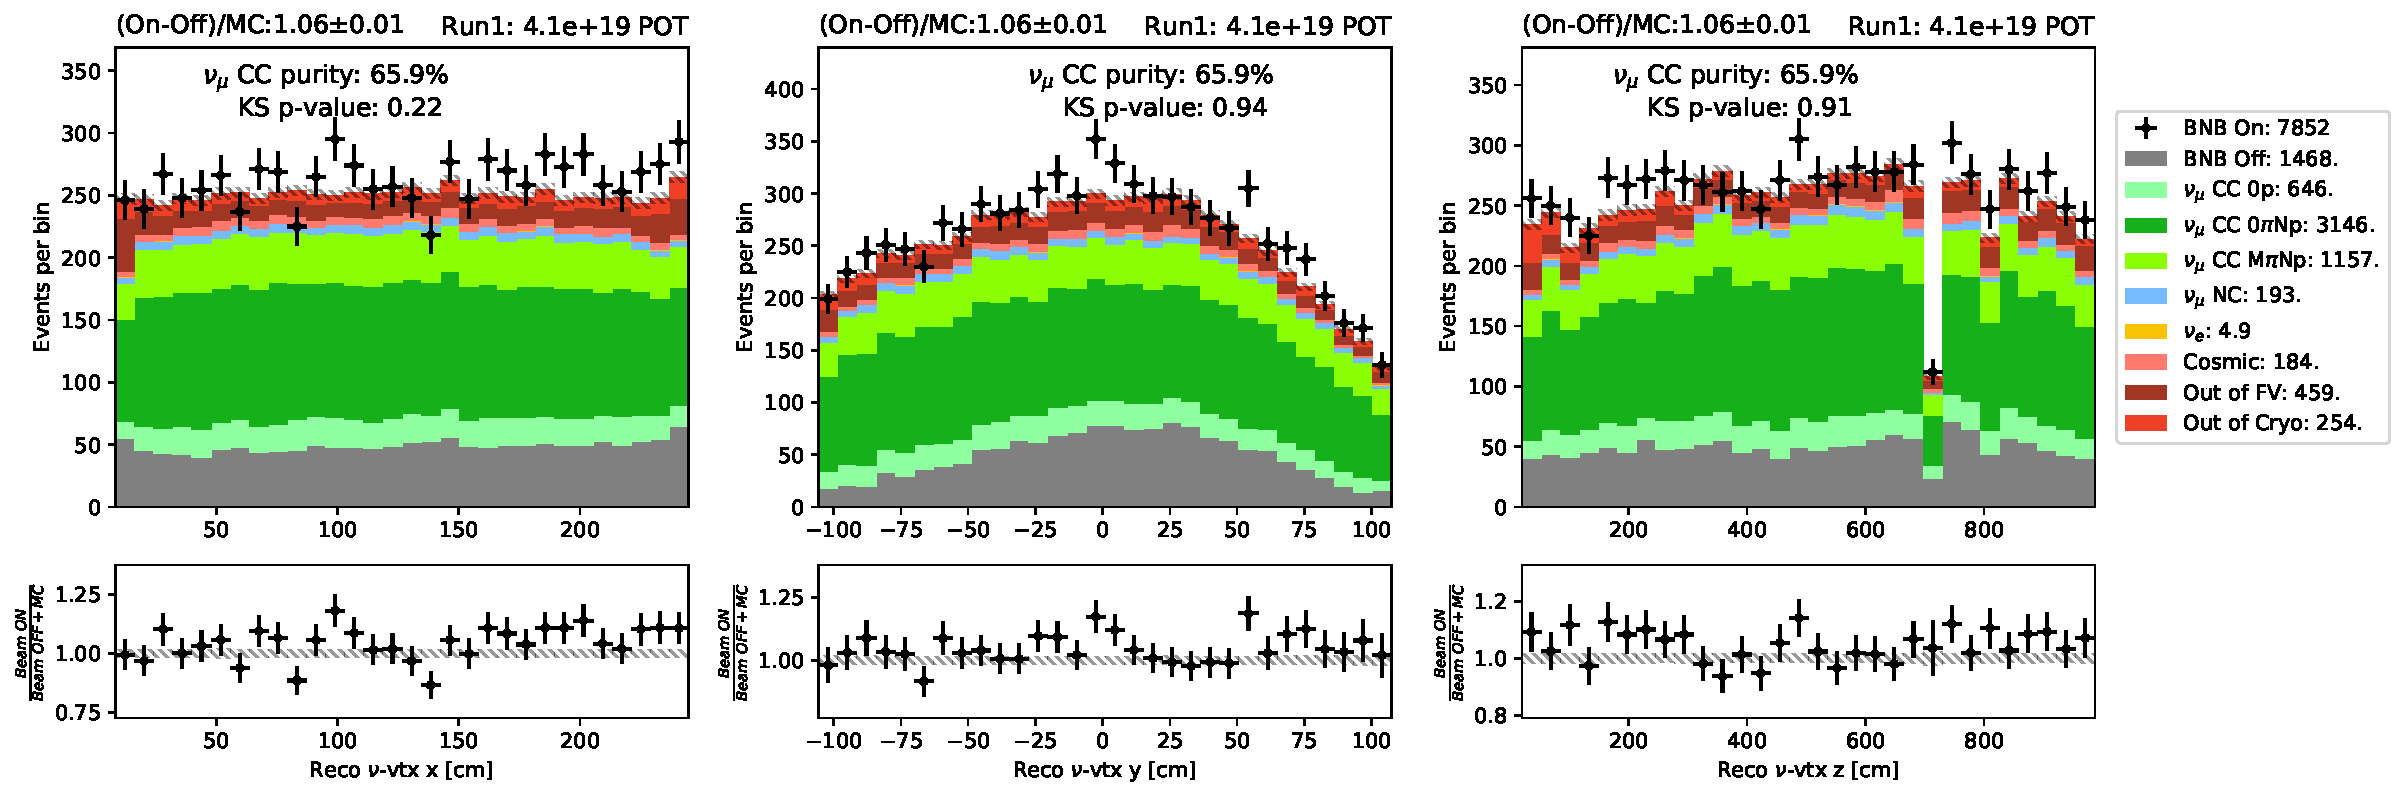
\includegraphics[width=\textwidth]{NuMuCCsel/Images/run1/numu_recovtx_run1.pdf}
    \caption{Caption}
    \label{fig:numu_vtx}
\end{figure}

\subsubsection{Run3}
\label{sssec:NuMUCCsel:INC:Run3}

\begin{figure}
    \centering
    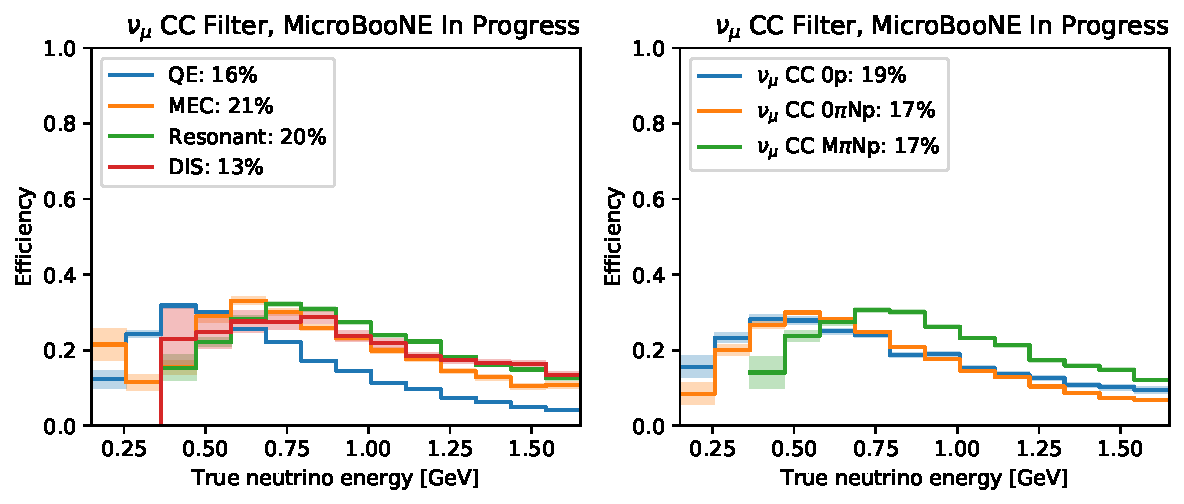
\includegraphics[width=0.85\textwidth]{NuMuCCsel/Images/run3/numu_efficiency_run3.pdf}
    \caption{Caption}
    \label{fig:numu_eff_r3}
\end{figure}


\begin{figure}
    \centering
    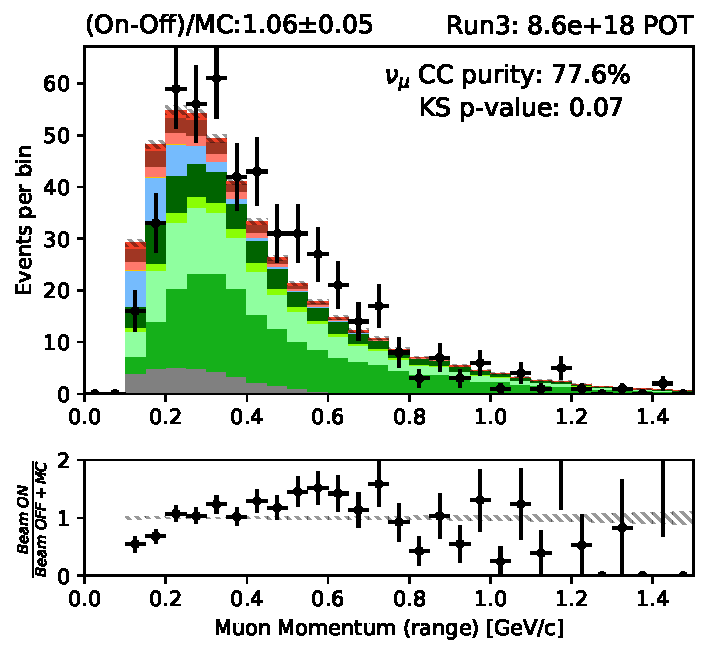
\includegraphics[height=6.5cm]{NuMuCCsel/Images/run3/numu_rangemom_run3.pdf} \hspace{2mm}
    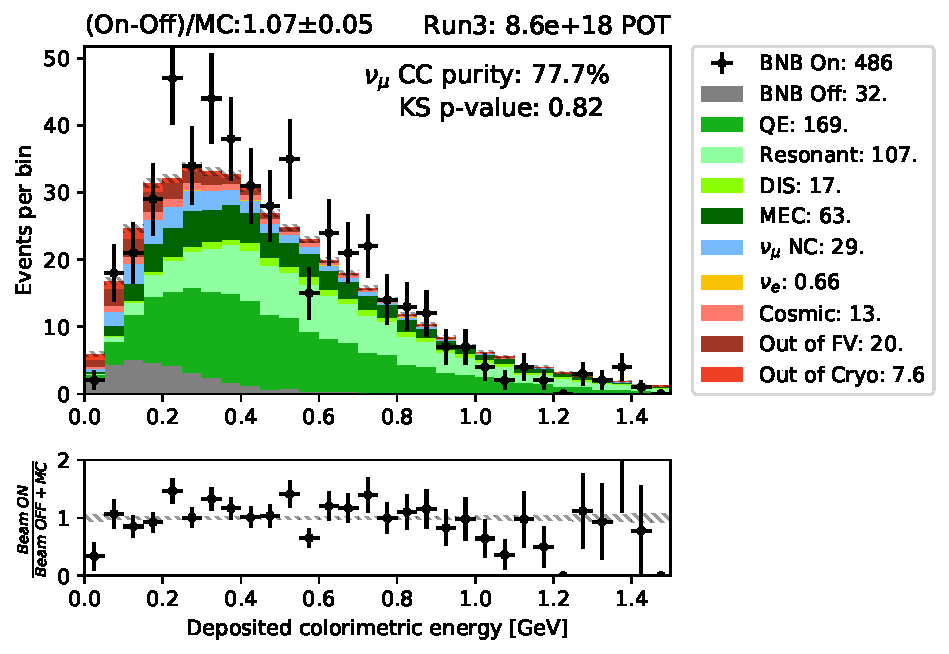
\includegraphics[height=6.5cm]{NuMuCCsel/Images/run3/numu_caloe_run3.pdf}
    \caption{Caption}
    \label{fig:numu_energy}
\end{figure}

\begin{figure}
    \centering
    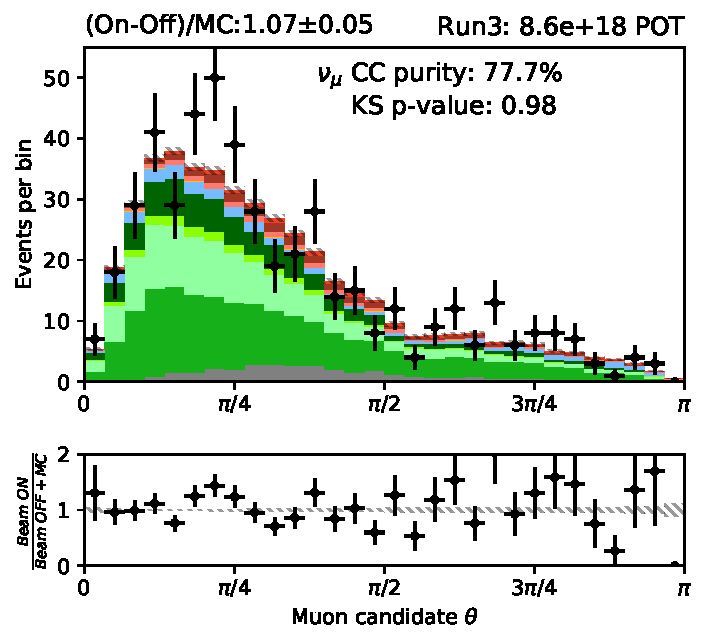
\includegraphics[height=6.5cm]{NuMuCCsel/Images/run3/numu_theta_run3.pdf} \hspace{2mm}
    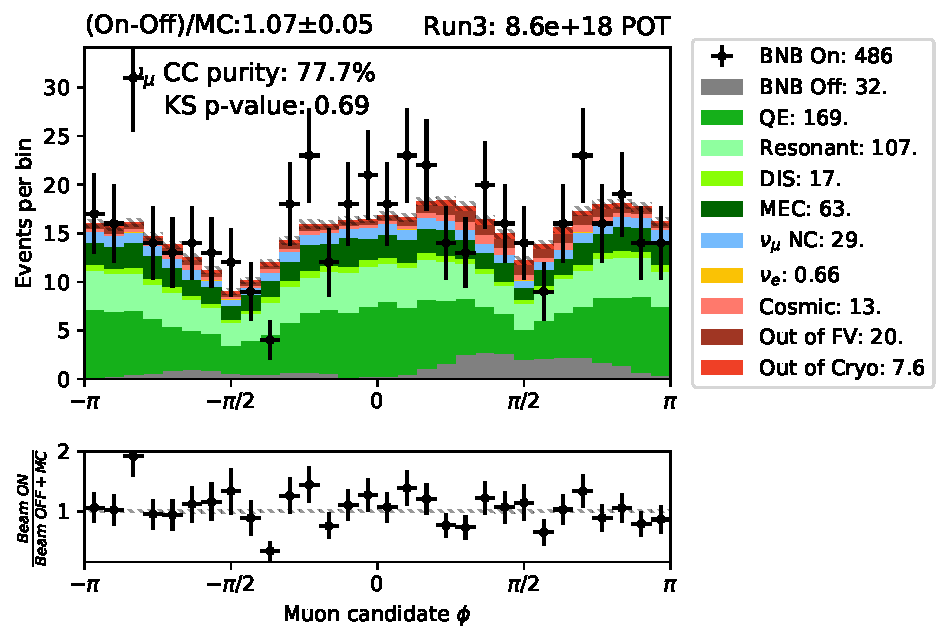
\includegraphics[height=6.5cm]{NuMuCCsel/Images/run3/numu_phi_run3.pdf}
    \caption{Caption}
    \label{fig:numu_angles}
\end{figure}

\subsection{$\nu_{\mu}$ Constraint \textcolor{red}{Ryan}}
\label{ssec:NuMUCCsel:constr}
\par The purpose of this $\nu_{\mu}$ side-band is to constrain the systematic uncertainties in the $\nu_{e}$ analysis. This is able to be done because the $\nu_{\mu}$s and $\nu_{e}$s of the BNB are subject to similar, correlated uncertainties, namely flux and cross-section modelling uncertainties. The $\nu_{e}$ selection is subject to higher uncertainties due to its low statistics. The $\nu_{\mu}$ component benefits from an order-of-magnitude advantage in absolute flux at MicroBooNE (Docdb 1031) and is exploited to constrain the uncertainties on the $\nu_{e}$s. For more information regarding the philosophy and goals of this constraint see sec \ref{ssec:goalsofnumusel}.

\par This selection prioritizes higher efficiencies and purities in the low-energy region that is the interest to the LEE analysis. Unfortunately, the flux and cross-section predictions for $\nu_{e}$ are most uncertain in the few-hundreds MeV energy region. Fortunately, the absolute $\nu_{\mu}$ flux (fig \ref{fig:bnb_absoluteflux}) and the cross-species flux correlation is greatest below 1 GeV (see figs \ref{fig:numuconstraint:flux}, \ref{fig:numuconstraint}).

\begin{figure}
    \centering
    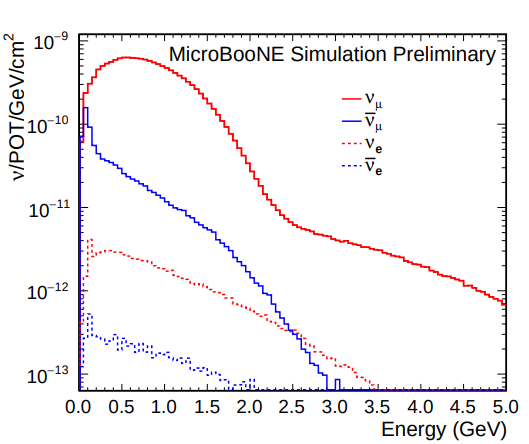
\includegraphics[height=6.5cm]{NuMuCCsel/Images/Ryan/absoluteFlux_uBooNE.png} \hspace{2mm}
    \caption{The absolute neutrino flux prediction through the MicroBooNE detector as calculated by the beam simulation. Shown is the flux for $\nu_{\mu}$, $\overline{\nu_{\mu}}$, $\nu_{e}$, and $\overline{\nu_{e}}$ averaged through the TPC volume with dimensions 2.56m by 2.33m by10.37m. DocDb 1031}
    \label{fig:bnb_absoluteflux}
\end{figure}

\subsubsection{Signal Definition}
\label{sssec:NuMUCCsel:constr:signaldef}
\par A $\nu_{\mu}$ event is identified by the presence of one muon candidate originating from inside the fiducial volume of the detector. Additional tracks and showers may accompany the muon candidate; these assist in reconstruction but are not necessary in the inclusive selection. Future studies of the $\nu_{\mu}$ side-band may require the presence of proton candidates to further constrain interaction models.

\subsubsection{Event Preselection}
\label{sssec:NuMUCCsel:constr:preselec}

\par The selection of $\nu_{\mu}$ events is built from the groundwork of the SliceID tool (see sec. \ref{sec:sliceID:SliceID}) and a combination of cuts on event-level and track-level observable values. The cuts in this section are primarily designed to eliminate cosmic and dirt backgrounds and select slices that are $\nu_{\mu}$-like. The methodology of this selection is similar to the selections in sec \ref{fig:nueselections} where first, the common SliceID filter is applied; next, event-level cuts are applied to select $\nu_{\mu}$-like events; finally, track-level cuts are applied to screen for muon-like candidates. The muon-candidate selection is described in sec \ref{sssec:NuMUCCsel:sel:muonsel}.

\par The requirement that the reconstructed vertex be contained inside the fiducial volume and that the slice have a sufficiently high topological score favor $\nu_{\mu}$ CC events and disfavor activity that is cosmogenic or dirt-like. Those cuts, specifically, are:

\begin{itemize}
    \item \emph{nslice} = 1.
    \item \emph{n\_tracks\_contained} $>$= 1.
    \item \emph{reco\_nu\_vtx\_sce\_x} $\in$ [5,251] cm.
    \item \emph{reco\_nu\_vtx\_sce\_y} $\in$ [-110,110] cm.
    \item \emph{reco\_nu\_vtx\_sce\_z} $\in$ [20,986] cm.
    \item \emph{topological\_score} $>$ 0.06.
    \item \emph{reco\_nu\_vtx\_sce\_z} $\not\in$ [675,775] cm.
\end{itemize}

\par \noindent This selection defines a unique fiducial volume compared to other selections, even in this analysis. See sec \ref{sssec:NuMUCCsel:constr:FV} for discussion of the determination of this boundary. The final cut on the $z$ coordinate is to ensure that it is not in the region of `dead wires' in the MicroBooNE detector, this is common practice within this analysis and the larger collaboration.

\par \noindent Run 3 has the additional power to leverage the CRT system to further limit cosmic contamination in the signal.

\textbf{Run 3 only:}
\begin{itemize}
    \item \emph{CRT Veto} != 1 or \emph{crthitpe} $<$ 100
    \item \emph{closestNuCosmicDist} $>$ 5 cm
\end{itemize}

\subsubsection{Muon Selection}
\label{sssec:NuMUCCsel:constr:muonsel}

\par After the event-level cuts are applied, the tracks in the slice are further analyzed to identify muon candidates. At least one reconstructed track in the event must satisfy all these criterion for the event to pass the selection. If an event has more than one muon candidate, then the longest is taken. Of the muon candidates that pass this selection, $\approx 94\%$ are, in simulation, muons from $\nu_{\mu}$ CC interactions.

\begin{itemize}
    \item \emph{trk\_sce\_start\_x} $\in$ [5,251] cm.
    \item \emph{trk\_sce\_start\_y} $\in$ [-110,110] cm.
    \item \emph{trk\_sce\_start\_z} $\in$ [20,986] cm.
    \item \emph{trk\_sce\_end\_x} $\in$ [5,251] cm.
    \item \emph{trk\_sce\_end\_y} $\in$ [-110,110] cm.
    \item \emph{trk\_sce\_end\_z} $\in$ [20,986] cm.
    \item \emph{trk\_llr\_pid\_score} $>$ 0.2.
    \item \emph{trk\_trk\_score} $>$ 0.8.
    \item \emph{trk\_trk\_length} $>$ 10 cm.
    \item \emph{trk\_trk\_distance} $<$ 4 cm.
    \item \emph{pfp\_generation} = 2.
\end{itemize}

\par \noindent The cuts made on the start and end points of the reconstructed tracks require that the track is fully contained inside the fiducial volume of the detector. This containment cut further reduces the primary background for this selection are is cosmic muons, originating from outside the detector. The containment requirement also motivates the use of range-based momentum calculations on all the muon candidates. Range-based momentum has been shown to have a high resolution, the independently calculated MCS-based momentum can be used as a quality check (see fig \ref{fig:numusel:momres}). The containment condition rejects many higher-energy $\nu_{\mu}$ events that might leave the detector, but it has a high efficiency in the lower energies.

\par The cut on the track distance requires that the reconstructed track be sufficiently close to the interaction vertex, this removes many in-time cosmic muons that are reconstructed as part of the event.

\par The cut on the log likelihood ratio pid score is to separate the muons from the protons among the PFParticle tracks in the passing slices. The track length cut further separates the muons from the protons which tend to have shorter track lengths. 

\par The track score cut ensures that the selected tracks are particularly track-like and this removes many particularly high energy, track-like electrons from the selection. Finally the PFParticle generation cut ensures that pandora recognizes that the track is a first daughter of the parent neutrino interaction. 

\begin{figure}
    \centering
    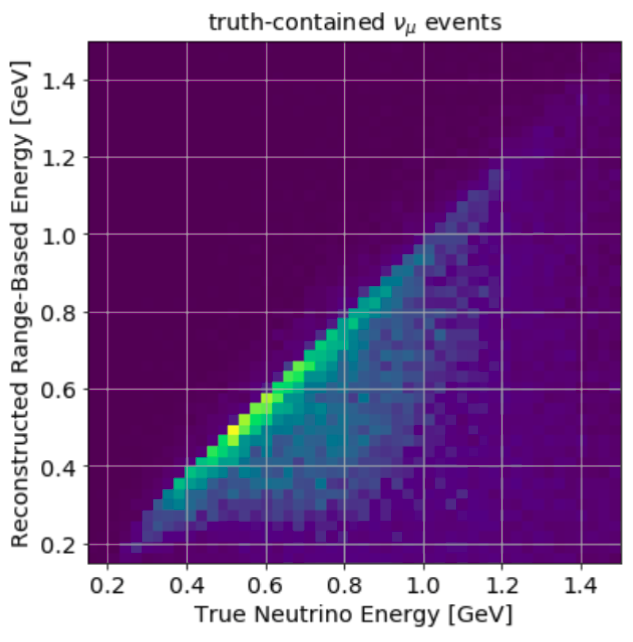
\includegraphics[height=6.5cm]{NuMuCCsel/Images/Ryan/containedMomentumRes.png} \hspace{2mm}
    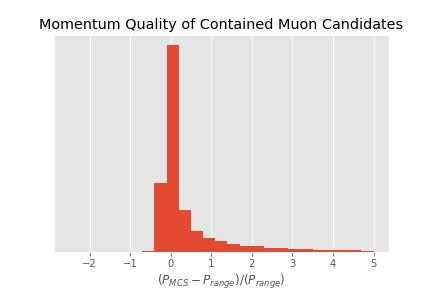
\includegraphics[height=6.5cm]{NuMuCCsel/Images/Ryan/muoncandidate_pquality.jpg} \hspace{2mm}
    \caption{The performance of range-based $\mu$ momentum calculation for contained tracks.}
    \label{fig:numusel:momres}
\end{figure}

\subsubsection{Determination of Fiducial Volume}
\label{sssec:NuMUCCsel:constr:FV}

\par The fiducial volume in this section differs slightly from other fiducial volumes, even in this analysis. Because the purpose of this selection is to leverage the high-statistics of the $\nu_{\mu}$ composition of the BNB, the fiducial volume is taken to be as large as possible while retaining high purity and efficiency at low-energies.

\par With the exception of the downstream fiducial volume face, all the fiducial volume boundaries are chosen in order to retain as many signal events as possible. The SCE-correction procedure is quite effective and can recover the true value give or take a few centimeters, with slightly less resolution near the boundaries. The resolution is shown in fig \ref{fig:NuMUCCsel:ryan:sceres_y} for the x-direction; the performance is similar in the x, y, and z directions. See fig \ref{fig:NuMUCCsel:ryan:FVhighy} for an example of signal purity near a boundary using the spacecharge-corrected coordinates. 

\begin{figure}
    \centering
    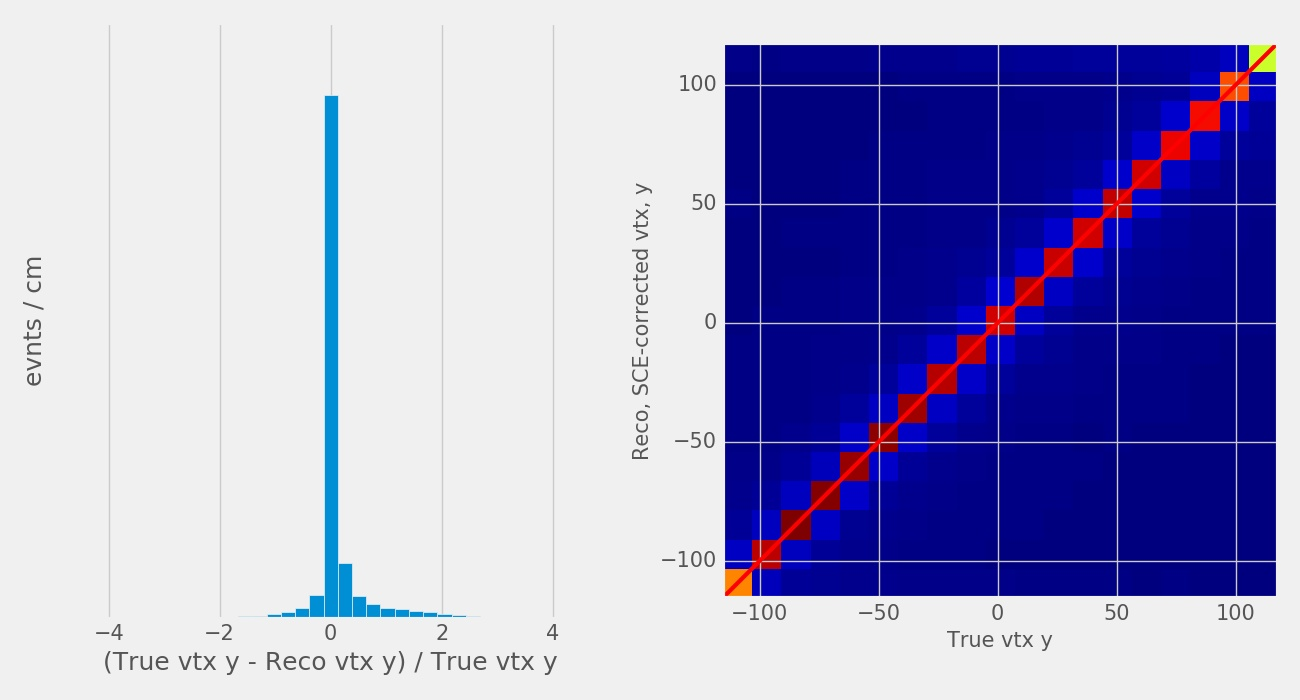
\includegraphics[height=6.5cm]{NuMuCCsel/Images/Ryan/sceresolution_y.jpg} \hspace{2mm}
    \caption{Resolution of the spacecharge-corrected vertex positions. The spacehcarge-corrected y-coordinates are being compared to the truth values without spacecharge distortion. }
    \label{fig:NuMUCCsel:ryan:sceres_y}
\end{figure}

\begin{figure}[ht] 
\begin{center}
    \begin{subfigure}[b]{0.45\textwidth}
    \centering
    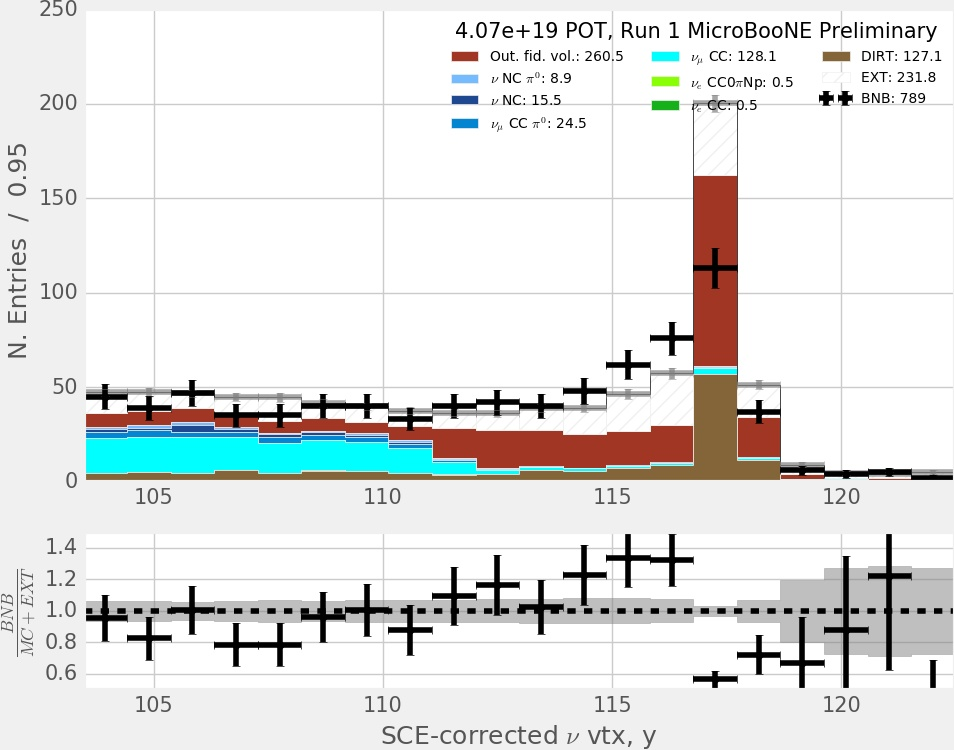
\includegraphics[width=1.00\textwidth]{NuMuCCsel/Images/Ryan/Run3_MCData_highy.jpg}
    \caption{\label{fig:NuMUCCsel:ryan:FVhighyMC} Data-MC distribution near top of detector.}
    \end{subfigure}
    \begin{subfigure}[b]{0.45\textwidth}
    \centering
    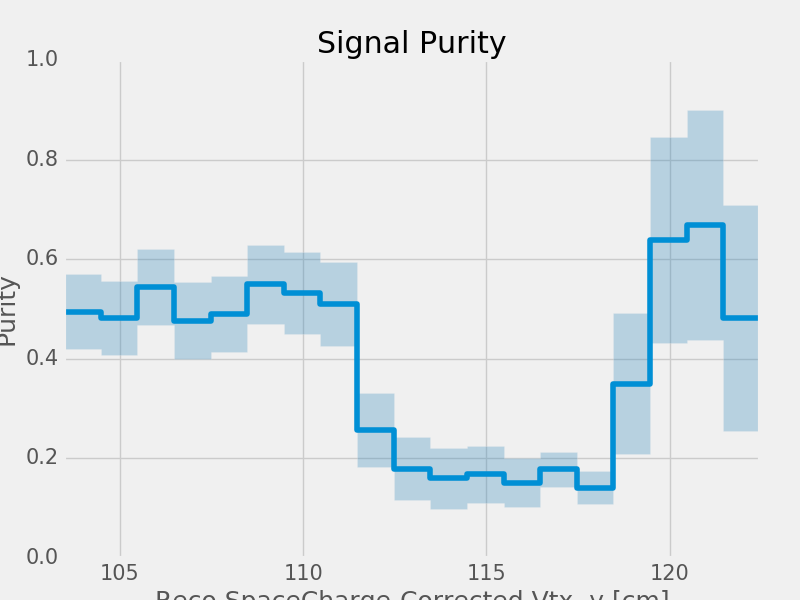
\includegraphics[width=1.00\textwidth]{NuMuCCsel/Images/Ryan/SignalPurity_highy.png}
    \caption{\label{fig:NuMUCCsel:ryan:FVhighyPur} Signal Purity}
    \end{subfigure}
\caption{Example of signal composition near boundary.}
\label{fig:NuMUCCsel:ryan:FVhighy}
\end{center}
\end{figure}

\subsubsection{Performance}
\label{sssec:NuMUCCsel:constr:performance}

\par This selection has been done on the Run1 and the Run3 sets processed for this analysis. The advantage of the Run1 data-set is higher statistics (5E19 POT in Run1 and 1E19 POT in Run3), but Run3 has the cosmic ray tagging system for extra background rejection. Distributions shown in this section will be of variables pertaining to the muon candidate for each event that passes the selection; Run1 data will be preferentially shown due to the higher statistics. The power of the Run3 CRT system will be demonstrated at the end of this section.

\par Run3 data includes information from the CRT system which was unavailable for the first MicroBooNE run. See fig \ref{fig:NuMUCCsel:ryan:Run3CRTcomp} for an example of the impact of the CRT. The CRT veto will eliminate more than 70$\%$ of the cosmics while suffering only roughly 15$\%$ loss in signal.

\par 

\begin{figure}[ht] 
\begin{center}
    \begin{subfigure}[b]{0.45\textwidth}
    \centering
    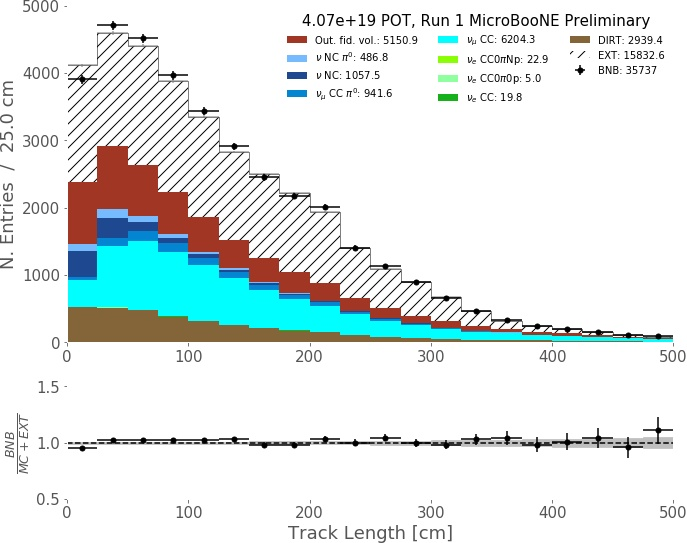
\includegraphics[width=1.00\textwidth]{NuMuCCsel/Images/Ryan/Run1_trklen_sliceID.jpg}
    \caption{\label{fig:NuMUCCsel:ryan:trklenSliceID} just sliceID}
    \end{subfigure}
    \begin{subfigure}[b]{0.45\textwidth}
    \centering
    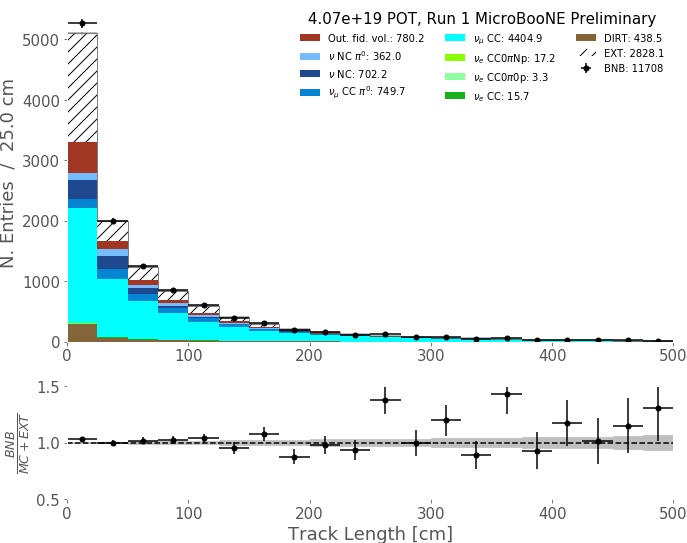
\includegraphics[width=1.00\textwidth]{NuMuCCsel/Images/Ryan/Run1_trklen_evtsel.jpg}
    \caption{\label{fig:NuMUCCsel:ryan:trklenEvt} just event-level preselection}
    \end{subfigure} \newline
    \begin{subfigure}[b]{0.45\textwidth}
    \centering
    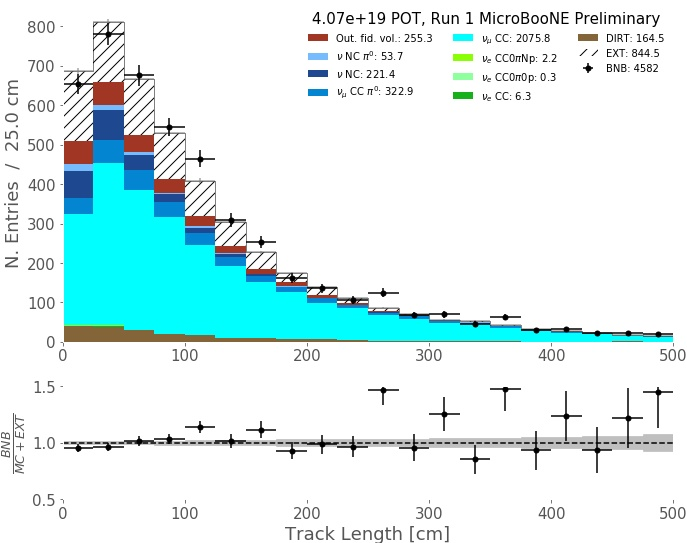
\includegraphics[width=1.00\textwidth]{NuMuCCsel/Images/Ryan/Run1_trklen_fullsel.jpg}
    \caption{\label{fig:NuMUCCsel:ryan:trklenFull} Full selection}
    \end{subfigure}
\caption{Track length of muon candidates. Just statistical uncertainties shown.}
\end{center}
\end{figure}

\begin{figure}[ht] 
\begin{center}
    \begin{subfigure}[b]{0.45\textwidth}
    \centering
    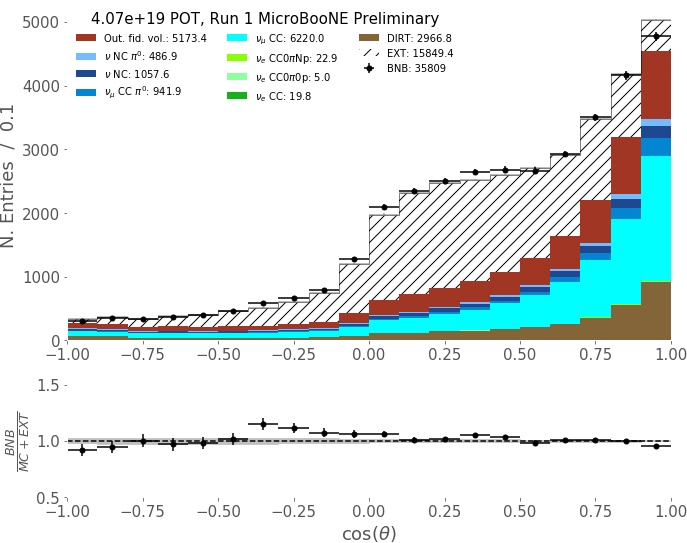
\includegraphics[width=1.00\textwidth]{NuMuCCsel/Images/Ryan/Run1_costheta_sliceID.jpg}
    \caption{\label{fig:NuMUCCsel:ryan:trklenSliceID} just sliceID}
    \end{subfigure}
    \begin{subfigure}[b]{0.45\textwidth}
    \centering
    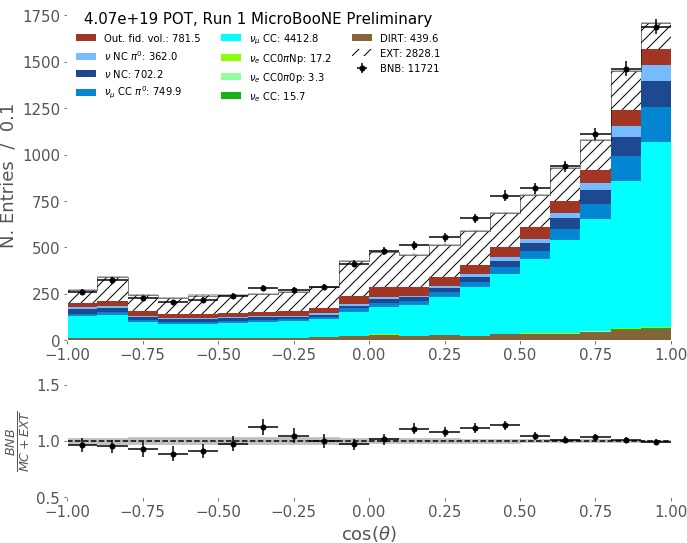
\includegraphics[width=1.00\textwidth]{NuMuCCsel/Images/Ryan/Run1_costheta_evtsel.jpg}
    \caption{\label{fig:NuMUCCsel:ryan:trklenEvt} just event-level preselection}
    \end{subfigure} \newline
    \begin{subfigure}[b]{0.45\textwidth}
    \centering
    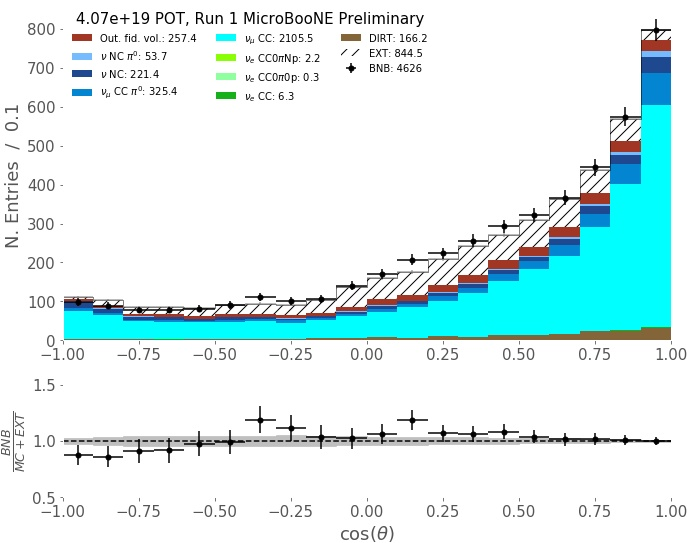
\includegraphics[width=1.00\textwidth]{NuMuCCsel/Images/Ryan/Run1_costheta_fullsel.jpg}
    \caption{\label{fig:NuMUCCsel:ryan:trklenFull} Full selection}
    \end{subfigure}
\caption{Cosine of the track angle of muon candidates with respect to the beam-direction. Just statistical uncertainties shown.}
\end{center}
\end{figure}

\begin{figure}[ht] 
\begin{center}
    \begin{subfigure}[b]{0.45\textwidth}
    \centering
    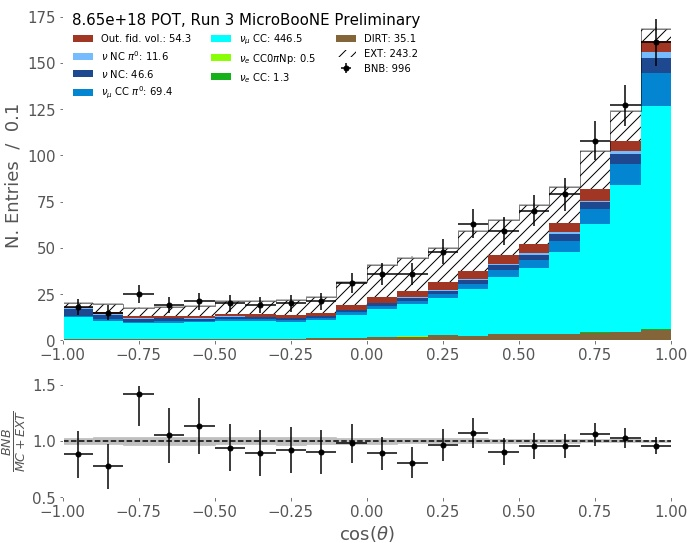
\includegraphics[width=1.00\textwidth]{NuMuCCsel/Images/Ryan/Run3_costheta_noCRT.jpg}
    \caption{\label{fig:NuMUCCsel:ryan:coswithCRT} without CRT}
    \end{subfigure}
    \begin{subfigure}[b]{0.45\textwidth}
    \centering
    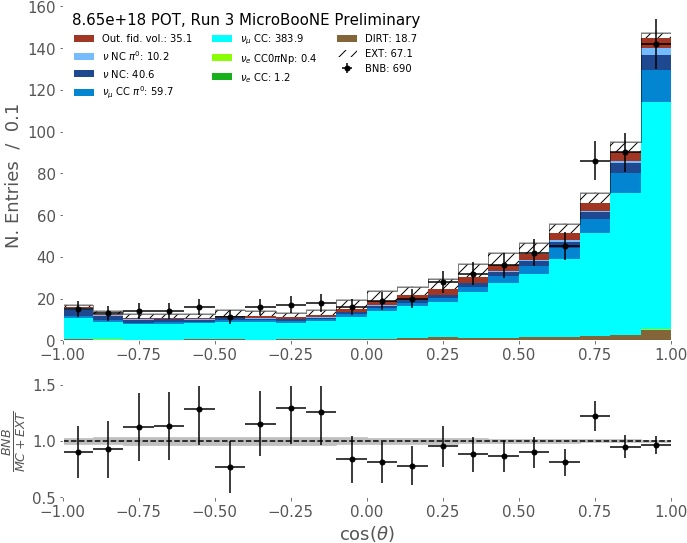
\includegraphics[width=1.00\textwidth]{NuMuCCsel/Images/Ryan/Run3_costheta_withCRT.jpg}
    \caption{\label{fig:NuMUCCsel:ryan:cosnoCRT} with CRT veto}
    \end{subfigure}
\caption{Angle with respect to the beam-direction of muon candidates for $\nu_{\mu}$ constraint. Just statistical uncertainties shown.}
\label{fig:NuMUCCsel:ryan:Run3CRTcomp}
\end{center}
\end{figure}